\documentclass[12pt,a4paper]{report}

%% --- Packages ---
\usepackage[a4paper, margin=2.5cm, headheight=15pt]{geometry}
\usepackage{graphicx}
\usepackage{float}
\usepackage{booktabs}
\usepackage{tabularx}
\usepackage{longtable}
\usepackage{multirow}
\usepackage{xcolor}
\usepackage{listings}
\usepackage{caption}
\usepackage{subcaption}
\usepackage{hyperref}
\usepackage{enumitem}
\usepackage{titlesec}
\usepackage{fancyhdr}
\usepackage{amsmath}
\usepackage{array}
\usepackage{colortbl}
\usepackage{setspace}
\usepackage{parskip}
\usepackage{tikz}
\usetikzlibrary{positioning}
\usepackage{mdframed}
\usepackage{fontawesome5}
\usepackage[utf8]{inputenc}
\usepackage[T1]{fontenc}
%\usepackage{lmodern}
%\usepackage{microtype}
\usepackage{tcolorbox}
\tcbuselibrary{skins,breakable}

%% --- Colours ---
\definecolor{primaryblue}{RGB}{25, 90, 170}
\definecolor{accentblue}{RGB}{66, 133, 244}
\definecolor{lightgray}{RGB}{245, 245, 245}
\definecolor{medgray}{RGB}{180, 180, 180}
\definecolor{darkgray}{RGB}{60, 60, 60}
\definecolor{successgreen}{RGB}{40, 167, 69}
\definecolor{warnorange}{RGB}{255, 140, 0}
\definecolor{errorred}{RGB}{220, 53, 69}
\definecolor{codebg}{RGB}{248, 248, 248}

%% --- Listings (code blocks) ---
\lstdefinestyle{jsonStyle}{
  backgroundcolor=\color{codebg},
  basicstyle=\ttfamily\small,
  breakatwhitespace=false,
  breaklines=true,
  captionpos=b,
  commentstyle=\color{gray},
  frame=single,
  rulecolor=\color{medgray},
  keywordstyle=\color{primaryblue}\bfseries,
  stringstyle=\color{successgreen},
  showstringspaces=false,
  tabsize=2
}
\lstdefinestyle{bashStyle}{
  backgroundcolor=\color{darkgray},
  basicstyle=\ttfamily\small\color{white},
  breakatwhitespace=false,
  breaklines=true,
  captionpos=b,
  frame=none,
  showstringspaces=false,
  tabsize=2
}
\lstset{style=jsonStyle}

%% --- Header / Footer ---
\pagestyle{fancy}
\fancyhf{}
\fancyhead[L]{\small\textcolor{primaryblue}{\textbf{Mini Distributed Cloud Object Store}}}
\fancyhead[R]{\small\textcolor{darkgray}{Cloud Computing Coursework Report}}
\fancyfoot[C]{\thepage}
\renewcommand{\headrulewidth}{0.5pt}
\renewcommand{\footrulewidth}{0pt}

%% --- Chapter / Section Formatting ---
\titleformat{\chapter}[display]
  {\normalfont\Large\bfseries\color{primaryblue}}
  {\chaptertitlename\ \thechapter}{10pt}{\Huge}
\titleformat{\section}
  {\normalfont\large\bfseries\color{primaryblue}}
  {\thesection}{1em}{}
\titleformat{\subsection}
  {\normalfont\normalsize\bfseries\color{darkgray}}
  {\thesubsection}{1em}{}
\titleformat{\subsubsection}
  {\normalfont\normalsize\itshape\color{darkgray}}
  {\thesubsubsection}{1em}{}

%% --- Hyperref Setup ---
\hypersetup{
  colorlinks=true,
  linkcolor=primaryblue,
  urlcolor=accentblue,
  citecolor=primaryblue,
  pdfauthor={Aayank Singhai},
  pdftitle={Mini Distributed Cloud Object Store --- Project Report},
  pdfsubject={Cloud Computing Coursework}
}

%% --- Custom Boxes ---
\newtcolorbox{infobox}[1][]{
  colback=accentblue!8,colframe=accentblue,
  title=#1,fonttitle=\bfseries,
  breakable
}
\newtcolorbox{keypoint}{
  colback=successgreen!8,colframe=successgreen,
  title=Key Design Point,fonttitle=\bfseries,
  breakable
}

%% --- Screenshot placeholder command ---
%% Usage: \screenshot{Caption text}{label}
\newcommand{\screenshot}[2]{%
  \begin{figure}[H]
    \centering
    \fbox{\begin{minipage}{0.92\textwidth}
      \vspace{1.5cm}
      \centering
      \textcolor{accentblue}{\Large\faCamera}\\[8pt]
      \textcolor{darkgray}{\small\textbf{[ Screenshot Placeholder ]}}\\[4pt]
      \textcolor{darkgray}{\footnotesize\textit{#1}}
      \vspace{1.5cm}
    \end{minipage}}
    \caption{#1}
    \label{fig:#2}
  \end{figure}
}

%% --- Double-screenshot side-by-side ---
\newcommand{\twoscreenshots}[4]{%
  \begin{figure}[H]
    \centering
    \begin{subfigure}[t]{0.48\textwidth}
      \fbox{\begin{minipage}{\textwidth}
        \vspace{1.2cm}
        \centering
        \textcolor{accentblue}{\faCamera}\\[4pt]
        \textcolor{darkgray}{\scriptsize\textbf{[ Screenshot ]}}\\[2pt]
        \textcolor{darkgray}{\tiny\textit{#1}}
        \vspace{1.2cm}
      \end{minipage}}
      \caption{#1}
      \label{fig:#2}
    \end{subfigure}
    \hfill
    \begin{subfigure}[t]{0.48\textwidth}
      \fbox{\begin{minipage}{\textwidth}
        \vspace{1.2cm}
        \centering
        \textcolor{accentblue}{\faCamera}\\[4pt]
        \textcolor{darkgray}{\scriptsize\textbf{[ Screenshot ]}}\\[2pt]
        \textcolor{darkgray}{\tiny\textit{#3}}
        \vspace{1.2cm}
      \end{minipage}}
      \caption{#3}
      \label{fig:#4}
    \end{subfigure}
  \end{figure}
}
      \label{fig:#4}
    \end{subfigure}
  \end{figure}
}

%% --- Document ---
\begin{document}

%% ---
%%  TITLE PAGE
%% ---
\begin{titlepage}
  \centering
  \vspace*{1cm}

  {\color{primaryblue}\rule{\linewidth}{2pt}}\\[0.6cm]

  {\Huge\bfseries\color{primaryblue} Mini Distributed Cloud\\[6pt]Object Store}\\[0.4cm]
  {\large\color{darkgray} Cloud Computing Coursework Project Report}\\[0.3cm]
  {\color{primaryblue}\rule{\linewidth}{1pt}}\\[1.5cm]

  %% Project logo / banner placeholder
  \begin{figure}[H]
    \centering
    \fbox{\begin{minipage}{0.75\textwidth}
      \vspace{2cm}
      \centering
      \textcolor{medgray}{\Huge\faCloud}\\[8pt]
      \textcolor{darkgray}{\small\textit{[ Project Architecture Banner / Screenshot ]}}
      \vspace{2cm}
    \end{minipage}}
  \end{figure}

  \vspace{1cm}

  {\large\bfseries Student Name:} \quad {\large Aayank Singhai}\\[0.3cm]
  {\large\bfseries Course:} \quad {\large Cloud Computing}\\[0.3cm]
  {\large\bfseries Academic Year:} \quad {\large 2025--2026}\\[0.3cm]
  {\large\bfseries Submission Date:} \quad {\large October 31, 2026}\\[0.3cm]

  \vfill

  {\color{primaryblue}\rule{\linewidth}{1pt}}\\[0.3cm]
  {\small\color{darkgray} All source code, Dockerfiles, demo scripts, and documentation are available\\
  in the project repository at:\\[4pt]
  \texttt{/home/aayanksinghai/Desktop/cloud/project/Mini Distributed Cloud Object Store/}}
\end{titlepage}

%% ---
%%  TABLE OF CONTENTS
%% ---
\tableofcontents
\newpage
\listoffigures
\newpage
\listoftables
\newpage

%% ---
%%  CHAPTER 1 --- INTRODUCTION
%% ---
\chapter{Introduction}

\section{Project Overview}

This report describes the design, implementation, and evaluation of the \textbf{Mini Distributed Cloud Object Store} --- a fully-featured, production-structured distributed storage system built as a Cloud Computing coursework project. The system replicates core concepts found in large-scale object storage services such as Amazon S3, Google Cloud Storage, and Azure Blob Storage, implemented from first principles without relying on managed cloud providers.

The system stores arbitrary binary objects by splitting them into fixed-size \textbf{1 MiB (1,048,576-byte) chunks}, distributing each chunk across multiple independent storage workers, and maintaining a \textbf{Replication Factor of 2 (RF = 2)} to ensure fault tolerance. It implements automatic failure detection, transparent read failover, re-replication after worker failures, rejoining reconciliation, and SHA-256 data integrity verification at both chunk and whole-object granularity.

\begin{infobox}[System at a Glance]
\begin{tabular}{ll}
\textbf{Controller:}       & 1 (Spring Boot 3.5.7, Java 21) \\
\textbf{Storage Workers:}  & 4 independent nodes \\
\textbf{Metadata Store:}   & PostgreSQL 16 \\
\textbf{Chunk Size:}       & 1 MiB (1,048,576 bytes) \\
\textbf{Replication:}      & RF = 2 on distinct workers \\
\textbf{Web Dashboard:}    & React 18 + TypeScript 5 + Vite 5 \\
\textbf{Deployment:}       & Docker \& Docker Compose (no Kubernetes) \\
\textbf{Integrity:}        & SHA-256 per-chunk + per-object \\
\end{tabular}
\end{infobox}

\section{Motivation}

Distributed object storage systems are foundational components of modern cloud infrastructure. Understanding and implementing core mechanisms --- including data sharding, replication, consistency, failure detection, and repair --- provides deep practical insight into distributed systems theory. This project was designed to demonstrate mastery of these concepts using realistic software engineering practices: multi-service containerisation, REST API design, structured error handling, automated testing, and observability.

\section{Objectives}

The primary objectives of this project are:

\begin{enumerate}[leftmargin=*, label=\textbf{O\arabic*.}]
  \item Implement a \textbf{RESTful object storage API} (`POST`, `GET`, `DELETE`, `LIST`, `GET metadata`, `PATCH metadata`) with structured JSON error responses.
  \item Split uploaded objects into \textbf{exact 1 MiB chunks} with deterministic chunk IDs and preserved ordering.
  \item Distribute chunks across \textbf{4 independent storage workers} with \textbf{RF = 2} on strictly distinct worker nodes.
  \item Detect worker failures via heartbeats and \textbf{automatically re-replicate} under-replicated chunks after a grace period.
  \item Perform \textbf{SHA-256 integrity verification} on every chunk read and repair corrupted replicas from healthy copies.
  \item Provide a \textbf{real-time web dashboard} for visual monitoring of objects, chunks, workers, replication status, and events.
  \item Package the entire system as a single \textbf{Docker Compose} stack runnable with one command.
  \item Cover all requirements with automated \textbf{unit, integration, and end-to-end tests}.
\end{enumerate}

\section{Report Structure}

This report is organised as follows:
\textbf{Chapter 2} presents the system architecture and design.
\textbf{Chapter 3} covers the technology stack.
\textbf{Chapter 4} describes the data model and storage design.
\textbf{Chapter 5} details the REST API specification.
\textbf{Chapter 6} explains core algorithms and workflows.
\textbf{Chapter 7} describes the web dashboard.
\textbf{Chapter 8} covers testing and verification.
\textbf{Chapter 9} documents the six demonstration scenarios from the coursework specification.
\textbf{Chapter 10} discusses design decisions and trade-offs.
\textbf{Chapter 11} concludes with a reflection and future work.

%% ---
%%  CHAPTER 2 --- SYSTEM ARCHITECTURE
%% ---
\chapter{System Architecture}

\section{High-Level Architecture}

The system follows a \textbf{centralised controller + distributed storage workers} architecture. The Controller is the single entry point for all client requests and manages all metadata in PostgreSQL. The four Storage Workers are entirely stateless with respect to metadata --- they only store raw chunk files on their local volumes and report liveness via periodic heartbeats.

\begin{figure}[H]
  \centering
  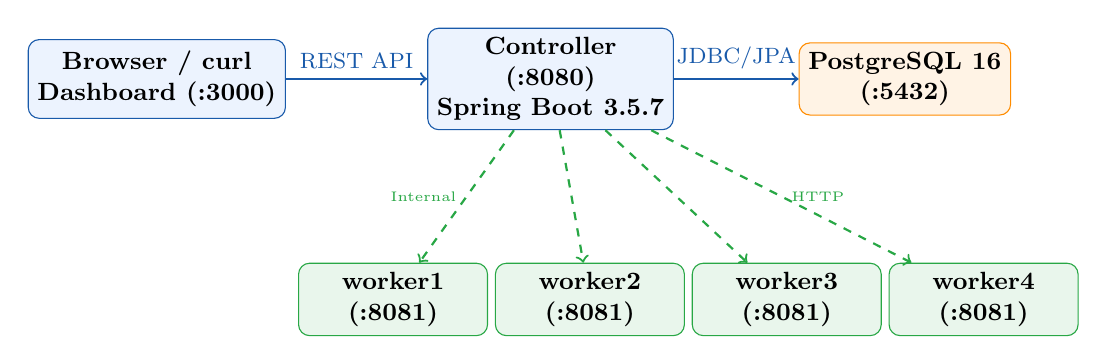
\begin{tikzpicture}[
    box/.style={draw=primaryblue, fill=accentblue!10, rounded corners=4pt,
                minimum width=3cm, minimum height=1cm, font=\small\bfseries, align=center},
    worker/.style={draw=successgreen, fill=successgreen!10, rounded corners=4pt,
                   minimum width=2.4cm, minimum height=0.9cm, font=\small\bfseries, align=center},
    db/.style={draw=warnorange, fill=warnorange!10, rounded corners=4pt,
               minimum width=2.6cm, minimum height=0.9cm, font=\small\bfseries, align=center},
    arr/.style={->, thick, color=primaryblue},
    iarr/.style={->, thick, color=successgreen, dashed}
  ]
    %% Client
    \node[box] (client) at (0,0) {Browser / curl\\Dashboard (:3000)};
    %% Controller
    \node[box] (ctrl) at (5,0) {Controller\\(:8080)\\Spring Boot 3.5.7};
    %% Postgres
    \node[db]  (pg)   at (9.5,0) {PostgreSQL 16\\(:5432)};
    %% Workers
    \node[worker] (w1) at (3,-2.8) {worker1\\(:8081)};
    \node[worker] (w2) at (5.5,-2.8) {worker2\\(:8081)};
    \node[worker] (w3) at (8,-2.8) {worker3\\(:8081)};
    \node[worker] (w4) at (10.5,-2.8) {worker4\\(:8081)};

    %% Arrows
    \draw[arr] (client) -- node[above, font=\footnotesize]{REST API} (ctrl);
    \draw[arr] (ctrl) -- node[above, font=\footnotesize]{JDBC/JPA} (pg);
    \draw[iarr] (ctrl) -- node[left, font=\tiny]{Internal} (w1);
    \draw[iarr] (ctrl) -- (w2);
    \draw[iarr] (ctrl) -- (w3);
    \draw[iarr] (ctrl) -- node[right, font=\tiny]{HTTP} (w4);
  \end{tikzpicture}
  \caption{High-level system architecture diagram.}
  \label{fig:arch-hld}
\end{figure}

\screenshot{Docker Compose cluster status showing all containers healthy (\texttt{docker-compose ps})}{compose-ps}

\section{Component Descriptions}

\subsection{Controller Service}

The Controller is the \textbf{brain} of the cluster. It is responsible for:
\begin{itemize}
  \item Accepting all client-facing REST API requests.
  \item Streaming uploaded objects through the \texttt{Chunker} and splitting into 1 MiB buffers.
  \item Maintaining all metadata in PostgreSQL (objects, chunks, replicas, workers, events, pending deletions).
  \item Selecting placement targets for chunk replicas using the \texttt{PlacementService} (least-loaded + rotating tie-break).
  \item Forwarding chunk bytes to selected workers in parallel using Java 21 virtual threads.
  \item Verifying SHA-256 checksums on chunk read and failing over to replica workers.
  \item Running scheduled background jobs: \texttt{HeartbeatMonitor}, \texttt{RepairScheduler}.
  \item Providing cluster-wide admin, replication repair, integrity scrubbing, and reconciliation APIs.
\end{itemize}

\subsection{Storage Workers (worker1--worker4)}

Each worker is an independent, stateless Spring Boot application that:
\begin{itemize}
  \item Accepts internal chunk \texttt{PUT / GET / DELETE} requests authenticated via \texttt{X-Internal-Token}.
  \item Stores chunks atomically: writes to a temp file, verifies SHA-256, \texttt{fsync}s, then \texttt{ATOMIC\_MOVE} to a two-level sharded path: \texttt{chunks/<2-hex-prefix>/<chunk\_id>.chunk}.
  \item Maintains a JSON sidecar file \texttt{<chunk\_id>.meta.json} with the expected SHA-256 checksum for on-disk verification.
  \item Runs a background \texttt{Scrubber} that periodically re-reads all stored chunks and reports corrupted ones via heartbeat.
  \item Sends periodic heartbeats to the Controller with liveness, storage metrics, and corrupt chunk IDs.
\end{itemize}

\subsection{PostgreSQL 16 (Metadata Store)}

The Controller persists all cluster metadata exclusively in PostgreSQL. No raw chunk bytes ever touch the Controller's or PostgreSQL's disk --- only structured metadata. The database is backed by the named Docker volume \texttt{postgres-data} for persistence across restarts.

\subsection{Web Dashboard}

A React 18 + TypeScript 5 + Vite 5 single-page application served by Nginx on port \texttt{3000}. Nginx reverse-proxies \texttt{/api/*} and \texttt{/actuator/*} requests to \texttt{controller:8080}, so the dashboard consumes real live API data with no backend of its own.

\section{Network Topology}

All containers communicate over a dedicated Docker bridge network \texttt{objectstore-net}. The Controller is the only container with an externally mapped port for client traffic (\texttt{:8080}). Workers are only reachable internally. The dashboard maps \texttt{:3000} externally and proxies API requests internally.

\begin{table}[H]
  \centering
  \caption{Container network and port mapping.}
  \label{tab:network}
  \begin{tabular}{llll}
    \toprule
    \textbf{Container} & \textbf{Image} & \textbf{Internal Port} & \textbf{Host Port} \\
    \midrule
    \texttt{postgres}    & \texttt{postgres:16-alpine}            & 5432 & --- (internal only) \\
    \texttt{controller}  & \texttt{objectstore/controller:latest} & 8080 & 8080 \\
    \texttt{worker1..4}  & \texttt{objectstore/worker:latest}     & 8081 & --- (internal only) \\
    \texttt{dashboard}   & \texttt{objectstore/dashboard:latest}  & 80   & 3000 \\
    \bottomrule
  \end{tabular}
\end{table}

\section{Persistent Storage Volumes}

A key architectural constraint is that every worker node has its own isolated, named Docker volume so chunk data persists across container restarts without interference between workers.

\begin{table}[H]
  \centering
  \caption{Named Docker volumes and mount paths.}
  \label{tab:volumes}
  \begin{tabular}{lll}
    \toprule
    \textbf{Volume Name}        & \textbf{Container}  & \textbf{Mount Path} \\
    \midrule
    \texttt{postgres-data}      & \texttt{postgres}   & \texttt{/var/lib/postgresql/data} \\
    \texttt{worker1-data}       & \texttt{worker1}    & \texttt{/data} \\
    \texttt{worker2-data}       & \texttt{worker2}    & \texttt{/data} \\
    \texttt{worker3-data}       & \texttt{worker3}    & \texttt{/data} \\
    \texttt{worker4-data}       & \texttt{worker4}    & \texttt{/data} \\
    \bottomrule
  \end{tabular}
\end{table}

%% ---
%%  CHAPTER 3 --- TECHNOLOGY STACK
%% ---
\chapter{Technology Stack}

\section{Backend (Controller \& Workers)}

\begin{table}[H]
  \centering
  \caption{Backend technology choices.}
  \label{tab:backend-stack}
  \begin{tabularx}{\textwidth}{llX}
    \toprule
    \textbf{Technology} & \textbf{Version} & \textbf{Role / Justification} \\
    \midrule
    Java          & 21 (LTS)   & Virtual threads (Project Loom) for parallel replica I/O without callback complexity; long-term support. \\
    Spring Boot   & 3.5.7      & Production-grade REST framework; autoconfiguration for JPA, Flyway, Jackson, multipart, Actuator. \\
    Spring Data JPA & 3.5.7   & Repository abstraction over Hibernate ORM; native SQL queries for placement and repair logic. \\
    Flyway        & 11.7.2     & Versioned, repeatable database migrations (\texttt{V1}--\texttt{V4}) applied atomically at startup. \\
    PostgreSQL    & 16         & ACID-compliant relational metadata store; row-level locking for optimistic concurrency on PATCH. \\
    HikariCP      & 6.3.3      & High-performance JDBC connection pool. \\
    Jackson       & 2.19       & JSON serialisation / deserialisation; used for API payloads and chunk sidecar metadata. \\
    Maven         & 3.9        & Multi-module build (\texttt{common}, \texttt{controller}, \texttt{worker}); offline reproducible builds via \texttt{-o}. \\
    \bottomrule
  \end{tabularx}
\end{table}

\section{Frontend (Web Dashboard)}

\begin{table}[H]
  \centering
  \caption{Frontend technology choices.}
  \label{tab:frontend-stack}
  \begin{tabularx}{\textwidth}{llX}
    \toprule
    \textbf{Technology} & \textbf{Version} & \textbf{Role} \\
    \midrule
    React         & 18.3.1  & Component-based SPA with concurrent rendering. \\
    TypeScript    & 5.9.3   & End-to-end static typing for API responses, component props, and state. \\
    Vite          & 5.4.21  & Sub-second HMR dev server; production bundle via Rollup. \\
    Nginx         & 1.27    & Static asset serving + \texttt{/api/*} reverse proxy to \texttt{controller:8080}. \\
    WebCrypto API & ---       & In-browser SHA-256 verification of downloaded objects (\texttt{crypto.subtle.digest}). \\
    \bottomrule
  \end{tabularx}
\end{table}

\section{Infrastructure \& Tooling}

\begin{table}[H]
  \centering
  \caption{Infrastructure and tooling.}
  \label{tab:infra-stack}
  \begin{tabularx}{\textwidth}{llX}
    \toprule
    \textbf{Tool}         & \textbf{Version} & \textbf{Purpose} \\
    \midrule
    Docker                & 24+     & Container runtime for all services. \\
    Docker Compose        & 2.x     & Single-command cluster orchestration (Kubernetes explicitly excluded per spec). \\
    JUnit 5               & 5.11    & Unit and integration test framework. \\
    AssertJ               & 3.27    & Fluent assertion DSL. \\
    Mockito               & 5.15    & Mock objects for unit tests. \\
    Testcontainers        & 1.21    & Real PostgreSQL container for integration tests (\texttt{@SpringBootTest}). \\
    WireMock              & 3.13    & HTTP stub server simulating 4 worker nodes in integration tests. \\
    Node Test Runner      & 20 (builtin) & Frontend unit tests without Vitest or Jest (all offline). \\
    esbuild               & (bundled) & TypeScript transpilation for dashboard unit tests. \\
    Bash / curl / jq      & ---       & Demo scripts and E2E test runner. \\
    \bottomrule
  \end{tabularx}
\end{table}

\section{Maven Multi-Module Structure}

The backend is organised as a Maven reactor with three modules sharing a common parent POM:

\begin{lstlisting}[style=bashStyle,caption=Maven module layout]
pom.xml                  (parent: Java 21, Spring Boot BOM 3.5.7)
--- common/pom.xml       (shared DTOs, error codes, exception hierarchy)
--- controller/pom.xml   (depends on common; full Spring Boot app)
--- worker/pom.xml       (depends on common; full Spring Boot app)
\end{lstlisting}

%% ---
%%  CHAPTER 4 --- DATA MODEL & STORAGE DESIGN
%% ---
\chapter{Data Model and Storage Design}

\section{Database Schema (PostgreSQL)}

The Controller persists four categories of data, versioned through four Flyway migrations:

\subsection{V1 --- Baseline Schema}
Establishes Flyway schema history baseline.

\subsection{V2 --- Workers and Events}

\begin{table}[H]
  \centering
  \caption{Table: \texttt{workers}}
  \label{tab:workers}
  \begin{tabular}{llll}
    \toprule
    \textbf{Column} & \textbf{Type} & \textbf{Constraints} & \textbf{Description} \\
    \midrule
    id               & \texttt{varchar}   & PK           & Worker identifier (\texttt{worker1}?\texttt{worker4}) \\
    endpoint\_url    & \texttt{varchar}   & NOT NULL     & Advertised HTTP base URL \\
    status           & \texttt{varchar}   & NOT NULL     & \texttt{UP} or \texttt{DOWN} \\
    total\_capacity  & \texttt{bigint}    & NOT NULL     & Total disk capacity in bytes \\
    used\_bytes      & \texttt{bigint}    & NOT NULL     & Used bytes as reported by heartbeat \\
    free\_bytes      & \texttt{bigint}    & NOT NULL     & Free bytes \\
    chunk\_count     & \texttt{int}       & NOT NULL     & Number of chunks stored \\
    last\_heartbeat  & \texttt{timestamp} &              & Last heartbeat received timestamp \\
    registered\_at  & \texttt{timestamp} & NOT NULL     & Initial registration timestamp \\
    \bottomrule
  \end{tabular}
\end{table}

\begin{table}[H]
  \centering
  \caption{Table: \texttt{system\_events}}
  \label{tab:events}
  \begin{tabular}{lll}
    \toprule
    \textbf{Column}   & \textbf{Type}      & \textbf{Description} \\
    \midrule
    id                & \texttt{bigint}    & Auto-increment PK \\
    event\_type       & \texttt{varchar}   & e.g. \texttt{WORKER\_DOWN}, \texttt{CHUNK\_REPAIRED} \\
    severity          & \texttt{varchar}   & \texttt{INFO}, \texttt{WARN}, \texttt{ERROR} \\
    message           & \texttt{text}      & Human-readable event description \\
    details           & \texttt{jsonb}     & Structured payload (worker ID, chunk ID, etc.) \\
    created\_at       & \texttt{timestamp} & Event timestamp \\
    \bottomrule
  \end{tabular}
\end{table}

\subsection{V3 --- Objects, Chunks, and Replicas}

\begin{table}[H]
  \centering
  \caption{Table: \texttt{objects}}
  \label{tab:objects-table}
  \begin{tabular}{lll}
    \toprule
    \textbf{Column}         & \textbf{Type}      & \textbf{Description} \\
    \midrule
    id                      & \texttt{uuid}      & Primary key (object ID) \\
    name                    & \texttt{varchar}   & Original filename \\
    size\_bytes             & \texttt{bigint}    & Total object size in bytes \\
    content\_type           & \texttt{varchar}   & MIME type \\
    checksum\_sha256        & \texttt{varchar}   & Whole-object SHA-256 (hex) \\
    chunk\_size\_bytes      & \texttt{bigint}    & Fixed chunk size (1,048,576) \\
    chunk\_count            & \texttt{int}       & Total number of chunks \\
    replication\_factor     & \texttt{int}       & Target RF (2) \\
    status                  & \texttt{varchar}   & \texttt{UPLOADING} or \texttt{ACTIVE} or \texttt{DELETING} \\
    version                 & \texttt{bigint}    & Optimistic locking version \\
    created\_at / updated\_at & \texttt{timestamp} & Lifecycle timestamps \\
    \bottomrule
  \end{tabular}
\end{table}

\begin{table}[H]
  \centering
  \caption{Table: \texttt{chunks} and \texttt{chunk\_replicas}}
  \label{tab:chunks}
  \begin{tabular}{lll}
    \toprule
    \textbf{Column}      & \textbf{Type}    & \textbf{Description} \\
    \midrule
    \multicolumn{3}{l}{\textit{\texttt{chunks}}} \\
    id                   & \texttt{varchar} & \texttt{\{objectId\}\_\{index:05d\}} \\
    object\_id           & \texttt{uuid}    & FK $\rightarrow$ \texttt{objects.id} \\
    chunk\_index         & \texttt{int}     & 0-based position in object \\
    size\_bytes          & \texttt{bigint}  & Actual chunk size in bytes \\
    checksum\_sha256     & \texttt{varchar} & Per-chunk SHA-256 (hex) \\
    \midrule
    \multicolumn{3}{l}{\textit{\texttt{chunk\_replicas}}} \\
    id                   & \texttt{uuid}    & Primary key \\
    chunk\_id            & \texttt{varchar} & FK $\rightarrow$ \texttt{chunks.id} \\
    worker\_id           & \texttt{varchar} & FK $\rightarrow$ \texttt{workers.id} \\
    state                & \texttt{varchar} & \texttt{HEALTHY}, \texttt{CORRUPTED}, \texttt{UNAVAILABLE} \\
    verified\_at         & \texttt{timestamp} & Last successful integrity check \\
    \bottomrule
  \end{tabular}
\end{table}

\subsection{V4 --- Pending Deletions Queue}

The \texttt{pending\_deletions} table holds deferred chunk deletion requests for workers that are \texttt{DOWN} at the time an object is deleted. When those workers rejoin, the reconciliation process executes all pending deletions.

\section{Worker On-Disk Storage Layout}

Each worker persists chunks using a two-level sharded directory to avoid inode exhaustion in a single directory:

\begin{lstlisting}[style=bashStyle, caption=Worker on-disk layout for a chunk]
/data/chunks/
--- temp/
---   --- <uuid>.tmp              # write-in-progress; deleted on success or crash
--- chunks/
    --- <2-hex-prefix>/
        --- <chunk_id>.chunk    # raw binary chunk bytes (exact 1 MiB or smaller final)
        --- <chunk_id>.meta.json  # {"chunkId":"...","checksumSha256":"...","sizeBytes":...}
\end{lstlisting}

The write protocol is strictly \textbf{write-to-temp $\rightarrow$ verify SHA-256 $\rightarrow$ fsync $\rightarrow$ ATOMIC\_MOVE}, preventing partial or corrupt writes from ever appearing in the \texttt{chunks/} directory.

\section{Chunk Identifier Design}

Chunk IDs are deterministically constructed as:
\[
  \text{chunkId} = \underbrace{\text{objectId}}_{\text{UUID}} \texttt{\_} \underbrace{\text{index}}_{\text{zero-padded 5 digits}}
\]

For example, the third chunk (index 2) of object \texttt{6b2c0a3a-9c77-4f8f-9a21-512e4ef63c01} has ID:
\[
  \texttt{6b2c0a3a-9c77-4f8f-9a21-512e4ef63c01\_00002}
\]

This format is \textbf{globally unique}, \textbf{lexically sortable} by chunk position, and \textbf{human-readable} in logs, worker directories, and the dashboard.

%% ---
%%  CHAPTER 5 --- REST API SPECIFICATION
%% ---
\chapter{REST API Specification}

\section{Client-Facing Object APIs}

All client APIs are served by the Controller on port \texttt{8080} under the prefix \texttt{/api/v1/}.

\begin{table}[H]
  \centering
  \caption{The 6 mandatory client-facing REST APIs.}
  \label{tab:client-apis}
  \begin{tabularx}{\textwidth}{llllX}
    \toprule
    \textbf{\#} & \textbf{Method} & \textbf{Path} & \textbf{Status} & \textbf{Description} \\
    \midrule
    1 & POST   & \texttt{/api/v1/objects}                       & 201 & Upload object (multipart: \texttt{file} + optional JSON \texttt{metadata}) \\
    2 & GET    & \texttt{/api/v1/objects/\{id\}}               & 200 & Stream reconstructed object with SHA-256 failover \\
    3 & GET    & \texttt{/api/v1/objects/\{id\}/metadata}      & 200 & Metadata + chunk/replica placement map \\
    4 & PATCH  & \texttt{/api/v1/objects/\{id\}/metadata}      & 200 & JSON Merge Patch custom metadata (no re-upload) \\
    5 & DELETE & \texttt{/api/v1/objects/\{id\}}               & 204 & Delete object + deferred deletions for DOWN workers \\
    6 & GET    & \texttt{/api/v1/objects}                      & 200 & Paginated, sortable object list \\
    \bottomrule
  \end{tabularx}
\end{table}

\subsection{Upload Response Body (201 Created)}
\begin{lstlisting}[style=jsonStyle, caption=Upload response --- ObjectInfo JSON]
{
  "objectId": "6b2c0a3a-9c77-4f8f-9a21-512e4ef63c01",
  "objectName": "demo.bin",
  "sizeBytes": 5557452,
  "contentType": "application/octet-stream",
  "checksumSha256": "e3b0c44298fc1c149afb...",
  "chunkSizeBytes": 1048576,
  "chunkCount": 6,
  "replicationFactor": 2,
  "status": "ACTIVE",
  "createdAt": "2026-10-31T10:00:00Z",
  "metadata": { "owner": "alice", "env": "prod" }
}
\end{lstlisting}

\section{Internal Controller--Worker APIs}

Internal APIs are authenticated with \texttt{X-Internal-Token: <INTERNAL\_API\_TOKEN>} (shared secret).

\begin{table}[H]
  \centering
  \caption{The 6 mandatory internal REST APIs.}
  \label{tab:internal-apis}
  \begin{tabularx}{\textwidth}{lllX}
    \toprule
    \textbf{Method} & \textbf{Path} & \textbf{Target} & \textbf{Description} \\
    \midrule
    POST   & \texttt{/internal/workers/register}             & Controller & Worker startup registration + auto-reconcile on rejoin \\
    POST   & \texttt{/internal/workers/heartbeat}            & Controller & Liveness, storage metrics, corruptChunkIds \\
    PUT    & \texttt{/internal/chunks/\{id\}}               & Worker     & Store chunk (verify \texttt{X-Chunk-Checksum} before commit) \\
    GET    & \texttt{/internal/chunks/\{id\}}               & Worker     & Read chunk with SHA-256 on-disk verification \\
    DELETE & \texttt{/internal/chunks/\{id\}}               & Worker     & Delete chunk and sidecar \\
    GET    & \texttt{/internal/workers/\{id\}/chunks}       & Worker/Ctrl & List chunks with optional verify + reconciliation diff \\
    \bottomrule
  \end{tabularx}
\end{table}

\section{Cluster, Admin, and Debug APIs}

\begin{table}[H]
  \centering
  \caption{Cluster and admin APIs.}
  \label{tab:admin-apis}
  \begin{tabularx}{\textwidth}{llX}
    \toprule
    \textbf{Method \& Path} & \textbf{Status} & \textbf{Description} \\
    \midrule
    \texttt{GET /api/v1/cluster/workers}           & 200 & All registered workers with health/capacity. \\
    \texttt{GET /api/v1/cluster/status}            & 200 & Cluster RF summary: healthy/degraded/unavailable/corrupted chunks. \\
    \texttt{POST /api/v1/admin/replication/repair} & 200 & Trigger immediate re-replication (bypasses grace period). \\
    \texttt{POST /api/v1/admin/workers/\{id\}/reconcile} & 200 & Full inventory reconciliation for one worker. \\
    \texttt{POST /api/v1/admin/integrity/scrub}    & 200 & SHA-256 scrub + optional repair across all UP workers. \\
    \texttt{POST /api/v1/admin/workers/\{wId\}/chunks/\{cId\}/corrupt} & 200 & Demo: proxy byte-flip corruption to worker. \\
    \texttt{GET /api/v1/admin/events}              & 200 & Paginated system event log with \texttt{since} cursor. \\
    \bottomrule
  \end{tabularx}
\end{table}

\section{Uniform Error Response Format}

Every error across both Controller and Worker returns a consistent JSON payload:

\begin{lstlisting}[style=jsonStyle, caption=Uniform ErrorResponse JSON format]
{
  "timestamp": "2026-10-31T10:05:12.345Z",
  "status": 404,
  "error": "Not Found",
  "code": "OBJECT_NOT_FOUND",
  "message": "Object not found: 6b2c0a3a-...",
  "path": "/api/v1/objects/6b2c0a3a-...",
  "details": {}
}
\end{lstlisting}

Defined error codes include: \texttt{OBJECT\_NOT\_FOUND}, \texttt{OBJECT\_NOT\_READY}, \texttt{CHUNK\_NOT\_FOUND}, \texttt{CHUNK\_CORRUPTED}, \texttt{CHUNK\_UNAVAILABLE}, \texttt{WORKER\_NOT\_FOUND}, \texttt{INSUFFICIENT\_STORAGE\_NODES}, \texttt{MISSING\_FILE}, \texttt{INVALID\_METADATA}, \texttt{CHECKSUM\_MISMATCH}.

%% ---
%%  CHAPTER 6 --- CORE ALGORITHMS AND WORKFLOWS
%% ---
\chapter{Core Algorithms and Workflows}

\section{Object Upload and 1 MiB Chunking}

\begin{figure}[H]
  \centering
  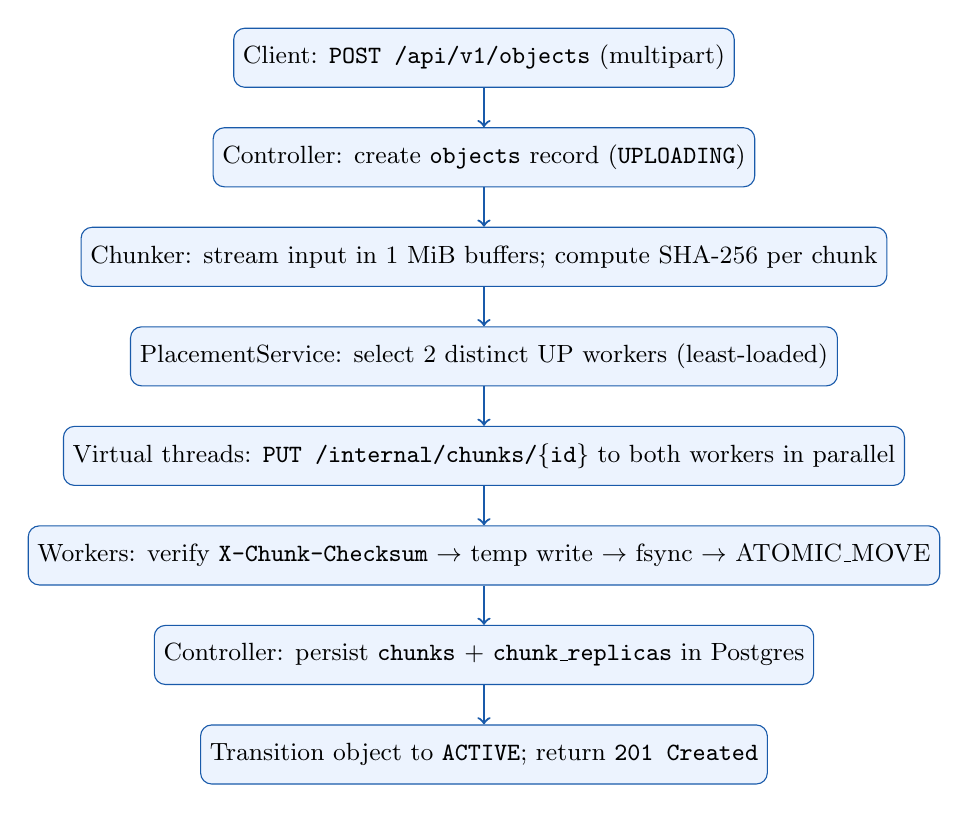
\begin{tikzpicture}[
    flowstep/.style={draw=primaryblue,fill=accentblue!10,rounded corners=4pt,
                 minimum width=5cm,minimum height=0.75cm,font=\small,align=center},
    arr/.style={->,thick,color=primaryblue}
  ]
    \node[flowstep] (s1) {Client: \texttt{POST /api/v1/objects} (multipart)};
    \node[flowstep, below=0.5cm of s1] (s2) {Controller: create \texttt{objects} record (\texttt{UPLOADING})};
    \node[flowstep, below=0.5cm of s2] (s3) {Chunker: stream input in 1 MiB buffers; compute SHA-256 per chunk};
    \node[flowstep, below=0.5cm of s3] (s4) {PlacementService: select 2 distinct UP workers (least-loaded)};
    \node[flowstep, below=0.5cm of s4] (s5) {Virtual threads: \texttt{PUT /internal/chunks/\{id\}} to both workers in parallel};
    \node[flowstep, below=0.5cm of s5] (s6) {Workers: verify \texttt{X-Chunk-Checksum} $\rightarrow$ temp write $\rightarrow$ fsync $\rightarrow$ ATOMIC\_MOVE};
    \node[flowstep, below=0.5cm of s6] (s7) {Controller: persist \texttt{chunks} + \texttt{chunk\_replicas} in Postgres};
    \node[flowstep, below=0.5cm of s7] (s8) {Transition object to \texttt{ACTIVE}; return \texttt{201 Created}};

    \foreach \a/\b in {s1/s2,s2/s3,s3/s4,s4/s5,s5/s6,s6/s7,s7/s8}
      \draw[arr] (\a) -- (\b);
  \end{tikzpicture}
  \caption{Object upload and chunking workflow.}
  \label{fig:upload-flow}
\end{figure}

\begin{keypoint}
The \textbf{Chunker} reads from the multipart \texttt{InputStream} in exact 1,048,576-byte buffers. The final chunk is whatever bytes remain (may be smaller). Both the per-chunk SHA-256 and the rolling whole-object SHA-256 are computed in a single streaming pass, keeping memory bounded at $O(\text{chunk\_size})$ regardless of object size.
\end{keypoint}

\section{Chunk Placement Algorithm}

The \texttt{PlacementService} selects 2 distinct worker targets for each chunk using:
\begin{enumerate}
  \item Filter to workers in \texttt{UP} state.
  \item Sort by \texttt{(chunk\_count ASC, used\_bytes ASC)} for load balancing.
  \item Apply a rotating cursor (round-robin tie-break) to ensure even chunk spread across all 4 workers.
  \item Enforce strict distinctness: the second target must not equal the first.
  \item If fewer than 2 UP workers exist, return \texttt{503 INSUFFICIENT\_STORAGE\_NODES}.
\end{enumerate}

\section{Object Download and Transparent Failover}

\begin{enumerate}[leftmargin=*]
  \item Verify the object is \texttt{ACTIVE}; check DB replica states.
  \item \textbf{Pre-flight check}: verify the first chunk has at least one reachable, non-corrupted replica before committing HTTP \texttt{200 OK} headers --- ensures a clean \texttt{503 CHUNK\_UNAVAILABLE} JSON response can still be returned if all replicas are corrupt.
  \item For each chunk ($i = 0$ to $n-1$):
    \begin{itemize}
      \item Order candidate replicas: \texttt{HEALTHY} on \texttt{UP} workers first.
      \item Request \texttt{GET /internal/chunks/\{id\}} from the best candidate.
      \item Worker re-reads the \texttt{.chunk} file and verifies SHA-256 against \texttt{.meta.json}.
      \item Controller re-verifies received bytes against Postgres \texttt{chunks.checksum\_sha256}.
      \item On mismatch or \texttt{409 CHUNK\_CORRUPTED}: mark that replica \texttt{CORRUPTED}, log \texttt{CHUNK\_CORRUPTED} event, and retry with the next candidate --- transparently.
    \end{itemize}
  \item Stream each verified chunk directly into the HTTP response body (\texttt{StreamingResponseBody}).
\end{enumerate}

\section{Worker Failure Detection and Re-Replication}

\begin{enumerate}[leftmargin=*]
  \item \textbf{HeartbeatMonitor} runs every \texttt{HEARTBEAT\_CHECK\_INTERVAL\_MS} (2s) and marks a worker \texttt{DOWN} if silent for $> $ \texttt{HEARTBEAT\_TIMEOUT\_MS} (10s).
  \item \texttt{ReconciliationService.handleWorkerDown} transitions all replicas on that worker to \texttt{UNAVAILABLE} and logs \texttt{WORKER\_DOWN} + \texttt{UNDER\_REPLICATED} events.
  \item \textbf{RepairScheduler} runs every \texttt{REPAIR\_INTERVAL\_MS} (10s). After \texttt{REREPLICATION\_GRACE\_PERIOD\_MS} (30s), \texttt{ReplicationService} re-replicates every chunk with $RF < 2$ by copying verified bytes from the surviving \texttt{HEALTHY} replica to a new distinct \texttt{UP} worker.
  \item When the failed worker restarts and re-registers, \texttt{reconcileWorker} runs automatically to: execute pending deletions, GC orphans, re-adopt valid replicas, and \textbf{trim surplus 3rd copies} to restore exact $RF = 2$.
\end{enumerate}

\section{SHA-256 Data Integrity Verification and Repair}

The system implements a \textbf{two-layer integrity model}:

\begin{table}[H]
  \centering
  \caption{Two-layer SHA-256 integrity checks.}
  \label{tab:integrity}
  \begin{tabularx}{\textwidth}{>{\bfseries}l X p{4.5cm}}
    \toprule
    \textbf{Layer} & \textbf{What is checked} & \textbf{Where Verified} \\
    \midrule
    Worker on-disk  & \texttt{.chunk} bytes vs. \texttt{.meta.json} checksum on every read & Worker \texttt{ChunkStore.get()} \\
    Controller receive & Received bytes vs. Postgres \texttt{chunks.checksum\_sha256} on every download & Controller \texttt{ObjectService} \\
    Background Scrubber & Re-reads all chunks periodically and reports \texttt{corruptChunkIds} via heartbeat & Worker \texttt{Scrubber} \\
    Admin scrub & \texttt{POST /api/v1/admin/integrity/scrub?repair=true} re-checks all UP workers and overwrites \texttt{CORRUPTED} replicas from healthy copies & Controller \texttt{IntegrityService} \\
    \bottomrule
  \end{tabularx}
\end{table}

%% ---
%%  CHAPTER 7 --- WEB DASHBOARD
%% ---
\chapter{Web Dashboard}

The dashboard is a React 18 + TypeScript 5 single-page application served by Nginx on port \texttt{3000}. It consumes all data from the live Controller REST API in real time and provides complete operational visibility into the cluster.

\section{Objects View}

\screenshot{Dashboard Objects page --- paginated and sortable object list with upload card}{dash-objects}

The Objects view provides:
\begin{itemize}
  \item \textbf{Drag-and-Drop Upload Card:} Drop any file, attach custom metadata key-value rows, and upload with a live progress bar.
  \item \textbf{Paginated, Sortable Object Table:} Sort by \texttt{createdAt}, \texttt{updatedAt}, \texttt{name}, or \texttt{size}. Download, inspect, or delete objects with confirmation.
\end{itemize}

\section{Object Detail View}

\screenshot{Dashboard Object Detail page --- chunk strip, replica matrix, and metadata editor}{dash-object-detail}

\twoscreenshots{ChunkStrip showing 6 ordered 1 MiB chunks, final chunk smaller}{dash-chunk-strip}{ReplicaMatrix (chunks $\times$ workers) coloured by HEALTHY/CORRUPTED/UNAVAILABLE state}{dash-replica-matrix}

The Object Detail view includes:
\begin{itemize}
  \item \textbf{In-Browser SHA-256 Verifier:} Click ``Verify Download SHA-256'' to stream the object through WebCrypto \texttt{crypto.subtle.digest} and compare against the stored \texttt{X-Object-Checksum-SHA256}.
  \item \textbf{Proportional Chunk Strip (\texttt{ChunkStrip}):} Renders ordered chunks with sizes proportional to their byte count, coloured by replication status.
  \item \textbf{Chunk $\times$ Worker Replica Matrix (\texttt{ReplicaMatrix}):} Interactive table mapping every chunk across \texttt{worker1}...\texttt{worker4}, with cell colours for \texttt{HEALTHY} (green), \texttt{CORRUPTED} (red), \texttt{UNAVAILABLE} (orange). Clicking a cell opens an action drawer with ``Corrupt this replica (demo)'' (when debug mode is enabled) and ``Scrub \& Repair Object''.
  \item \textbf{Live Metadata Editor:} Sends \texttt{PATCH} requests to add, update, or null-delete metadata keys in real time.
\end{itemize}

\section{Cluster View}

\screenshot{Dashboard Cluster page --- 4 Worker cards, cluster RF summary, and admin action buttons}{dash-cluster}

The Cluster view includes:
\begin{itemize}
  \item \textbf{Cluster Replication Banner:} Live counts of active objects, healthy/degraded/unavailable/corrupted chunks.
  \item \textbf{4 Worker Node Cards (\texttt{WorkerCard}):} \texttt{UP}/\texttt{DOWN} badge, heartbeat age, stored chunk count, used/total capacity bar, per-worker ``Reconcile Inventory'' button.
  \item \textbf{Admin Action Buttons:} One-click ``Run Replication Repair Now'' and ``Run Integrity Scrub (SHA-256)''.
\end{itemize}

\section{Operations Log View}

\screenshot{Dashboard Events page --- live system event log with severity and type filters}{dash-events}

The Operations Log view polls \texttt{GET /api/v1/admin/events} with a \texttt{since} cursor for live event streaming, displaying all 11 event types with severity badges and free-text search/filter.

%% ---
%%  CHAPTER 8 --- TESTING AND VERIFICATION
%% ---
\chapter{Testing and Verification}

\section{Testing Strategy}

The system is covered at five levels:

\begin{table}[H]
  \centering
  \caption{Multi-level testing strategy.}
  \label{tab:testing}
  \begin{tabularx}{\textwidth}{>{\bfseries}l p{4.2cm} X}
    \toprule
    \textbf{Level} & \textbf{Testing Tools} & \textbf{Scope and Coverage} \\
    \midrule
    Unit            & JUnit 5, AssertJ, Mockito  & \texttt{Chunker} boundary conditions (0 B, 1 B, 1 MiB-1, 1 MiB, 1 MiB+1, multi-chunk), SHA-256 correctness, placement distinctness and spread, merge-patch semantics, replica state transitions, chunk ID validation. \\
    Slice           & \texttt{@WebMvcTest}       & HTTP status codes, JSON error body structure, multipart validation. \\
    Integration     & Spring Boot Test, Testcontainers, WireMock & Upload round-trip, download with SHA-256 failover, concurrent 8-thread uploads, worker failure and reconciliation, corruption detection and repair, metadata PATCH lifecycle. \\
    Worker          & \texttt{@TempDir}, MockMvc & Atomic writes, checksum rejection, corrupt-on-read detection, inventory listing. \\
    End-to-End      & Bash, \texttt{curl}, \texttt{jq}, \texttt{sha256sum} & All 6 coursework scenarios (\S10.1--\S10.6) as asserting scripts + volume persistence across restart. \\
    Frontend        & Node 20 test runner, esbuild & Formatting helpers, metadata validation, replica matrix rendering, event deduplication, typed API client. \\
    \bottomrule
  \end{tabularx}
\end{table}

\section{Test Results}

\begin{table}[H]
  \centering
  \caption{Complete test suite results.}
  \label{tab:test-results}
  \begin{tabular}{lrrr}
    \toprule
    \textbf{Module} & \textbf{Tests} & \textbf{Passed} & \textbf{Failed} \\
    \midrule
    \texttt{common}      & 13 & 13 & 0 \\
    \texttt{controller}  & 35 & 35 & 0 \\
    \texttt{worker}      & 15 & 15 & 0 \\
    \midrule
    \textbf{Backend Total} & \textbf{63} & \textbf{63} & \textbf{0} \\
    \midrule
    \texttt{dashboard} (frontend) & 8 & 8 & 0 \\
    \midrule
    \textbf{Grand Total} & \textbf{71} & \textbf{71} & \textbf{0} \\
    \bottomrule
  \end{tabular}
\end{table}

\screenshot{Maven build output showing 63/63 backend tests passing (\texttt{mvn -B verify})}{mvn-test-results}

\screenshot{Frontend test run output showing 8/8 dashboard tests passing (\texttt{npm test})}{npm-test-results}

\section{Key Integration Tests}

\begin{itemize}
  \item \textbf{\texttt{ObjectUploadIntegrationTest}:} Multi-chunk upload (~2.48 MiB), 0-byte upload, single-worker write failover, $<$2 UP workers 503, and 400 validation errors.
  \item \textbf{\texttt{ObjectDownloadIntegrationTest}:} ~3.2 MiB 4-chunk binary round-trip SHA-256 equality, 0-byte file, transparent failover on worker DOWN or corrupted bytes, and all error paths.
  \item \textbf{\texttt{ReplicationIntegrationTest}:} 10 MiB / 10-chunk distinctness and even 4-worker distribution, grace period and re-replication, in-place CORRUPTED replica repair.
  \item \textbf{\texttt{WorkerFailureAndReconciliationIntegrationTest}:} Worker DOWN replica transition, byte-identical download from surviving replicas, full failure + re-replication + deferred deletion + rejoin trimming to exact RF = 2.
  \item \textbf{\texttt{DataIntegrityAndRecoveryIntegrationTest}:} Corruption on read + failover + repair, proactive scrub bit-rot detection and auto-repair, heartbeat corrupt reporting, 503 when all replicas corrupted.
  \item \textbf{\texttt{ConcurrencyAndEdgeCasesIntegrationTest}:} 8 concurrent multi-chunk uploads using virtual threads, sequential metadata patches + deletion, admin 404 error paths.
\end{itemize}

%% ---
%%  CHAPTER 9 --- DEMONSTRATION SCENARIOS
%% ---
\chapter{Demonstration Scenarios (Coursework Specification \S10)}

All six mandatory evaluation scenarios defined in Section 10 of the coursework specification (\texttt{Mini\_Distributed\_Cloud\_Object\_Store.pdf}) are fully automated as individual bash test scripts in \texttt{scripts/demo/01-object-storage.sh} through \texttt{06-data-integrity.sh}, and orchestrated end-to-end by \texttt{scripts/e2e/run-all.sh}.

\section{Scenario 1: Object Storage (Coursework \S10.1)}
\label{sec:demo-10-1}

\begin{infobox}[Demonstration Scenario Summary --- \S10.1 Object Storage]
\begin{tabularx}{\textwidth}{lX}
\textbf{Requirement:}      & Ingest arbitrary binary object $\rightarrow$ stream download $\rightarrow$ assert byte-identical hash equality. \\
\textbf{Automated Script:} & \texttt{scripts/demo/01-object-storage.sh} \\
\textbf{Primary APIs:}     & \texttt{POST /api/v1/objects}, \texttt{GET /api/v1/objects/\{objectId\}} \\
\textbf{Acceptance Test:}  & HTTP \texttt{201 Created} on upload; HTTP \texttt{200 OK} on download; $\text{SHA-256}_{\text{orig}} \equiv \text{SHA-256}_{\text{down}}$. \\
\end{tabularx}
\end{infobox}

\subsection{Objective and Context}
This demonstration verifies the primary functional contract of the object storage service: an arbitrary multi-megabyte binary payload is uploaded via multipart HTTP, ingested, chunked into 1~MiB segments, replicated across storage workers, and subsequently downloaded via streaming reassembly such that the reconstructed file is bit-for-bit identical to the original input.

\subsection{Demonstration Procedure}
The demonstration executes the following four-stage sequence:
\begin{enumerate}[leftmargin=*]
  \item \textbf{Payload Generation:} Generate a deterministic 2,465,792-byte ($\approx 2.35$~MiB) binary test file using pseudo-random bytes and compute its baseline SHA-256 digest:
\begin{lstlisting}[style=bashStyle]
head -c 2465792 /dev/urandom > /tmp/demo1.bin
ORIG_SHA=$(sha256sum /tmp/demo1.bin | awk '{print $1}')
\end{lstlisting}
  \item \textbf{Object Ingestion:} Upload the file via \texttt{POST /api/v1/objects} with custom metadata:
\begin{lstlisting}[style=bashStyle]
curl -s -X POST http://localhost:8080/api/v1/objects \
  -F "file=@/tmp/demo1.bin;filename=demo1.bin;type=application/octet-stream" \
  -F 'metadata={"scenario":"10.1","test":"object-storage"}'
\end{lstlisting}
  The Controller creates an \texttt{ACTIVE} object record, streams 3 chunks (two 1~MiB chunks and one 368,640-byte chunk) in parallel to distinct workers, and returns \texttt{201 Created} containing the \texttt{objectId} and server-computed \texttt{checksumSha256}.
  \item \textbf{Streaming Retrieval:} Download the object via \texttt{GET /api/v1/objects/\{objectId\}}:
\begin{lstlisting}[style=bashStyle]
curl -s -D /tmp/headers.txt http://localhost:8080/api/v1/objects/$OBJ_ID \
  -o /tmp/demo1.downloaded.bin
\end{lstlisting}
  The Controller streams the ordered chunks directly to the response body while verifying each chunk's SHA-256 on the fly.
  \item \textbf{Integrity Assertion:} Compute the SHA-256 hash of the downloaded file and assert strict three-way equality:
\[
  \text{SHA-256}(\text{original}) \;=\; \text{SHA-256}(\text{controller metadata}) \;=\; \text{SHA-256}(\text{downloaded})
\]
\end{enumerate}

\screenshot{Terminal execution output for Demonstration \S10.1 showing matching SHA-256 checksums and HTTP 200 headers}{demo-01-sha256}

\subsection{Verification and Expected Results}
\begin{itemize}[leftmargin=*]
  \item The upload returns HTTP \texttt{201 Created} with header \texttt{Location: /api/v1/objects/<objectId>}.
  \item The response JSON reports \texttt{chunkCount: 3}, \texttt{replicationFactor: 2}, and \texttt{status: "ACTIVE"}.
  \item The download response returns HTTP \texttt{200 OK} with headers:
    \begin{itemize}
      \item \texttt{Content-Type: application/octet-stream}
      \item \texttt{Content-Length: 2465792}
      \item \texttt{Content-Disposition: attachment; filename="demo1.bin"}
      \item \texttt{X-Object-Checksum-SHA256: <64-hex-digest>}
      \item \texttt{ETag: "<64-hex-digest>"}
    \end{itemize}
  \item The downloaded file size exactly matches the uploaded size, and \texttt{sha256sum} confirms zero bit corruption across all chunks.
\end{itemize}

\section{Scenario 2: Chunking and Distribution (Coursework \S10.2)}
\label{sec:demo-10-2}

\textbf{Objective:} Prove that a $\approx 5.3$~MiB file is split into exact 1~MiB chunks (last chunk smaller) distributed across all 4 workers.

\textbf{Procedure:}
\begin{enumerate}
  \item Upload a 5,557,452-byte binary file.
  \item Inspect \texttt{GET /api/v1/objects/\{objectId\}/metadata}: verify \texttt{chunkCount = 6}, chunk indices 0--4 each \texttt{sizeBytes = 1,048,576}, chunk index 5 \texttt{sizeBytes = 314,572}.
  \item Verify that all 4 workers (\texttt{worker1}--\texttt{worker4}) appear as replica holders across the 6 chunks.
  \item Inspect on-disk chunk files via \texttt{docker exec worker1 find /data/chunks -name "<objectId>\_*.chunk"}.
\end{enumerate}

\screenshot{Metadata API response showing 6 chunks, correct sizes, and 4-worker distribution}{demo-02-chunk-metadata}

\screenshot{Terminal showing \texttt{docker exec} output of .chunk files inside worker containers}{demo-02-docker-exec}

\textbf{Expected result:} 6 chunks, 5 $\times$ 1,048,576 bytes + 1 $\times$ 314,572 bytes; chunks distributed across all 4 workers.

\section{Scenario 3: Replication Verification (Coursework \S10.3)}
\label{sec:demo-10-3}

\textbf{Objective:} Prove that every chunk has exactly 2 \texttt{HEALTHY} replicas on distinct worker nodes.

\textbf{Procedure:}
\begin{enumerate}
  \item Inspect the metadata response for each chunk: verify \texttt{replicas} array has exactly 2 entries with distinct \texttt{workerId} values and \texttt{state: "HEALTHY"}.
  \item Call \texttt{GET /api/v1/cluster/status} and verify \texttt{underReplicatedChunks = 0} and \texttt{unavailableChunks = 0}.
\end{enumerate}

\screenshot{Cluster status API response showing 0 under-replicated and 0 unavailable chunks}{demo-03-cluster-status}

\section{Scenario 4: Metadata Operations and Lifecycle (Coursework \S10.4)}
\label{sec:demo-10-4}

\textbf{Objective:} Prove custom metadata can be added, updated, and deleted without re-uploading any chunk data.

\textbf{Procedure:}
\begin{enumerate}
  \item Upload with initial metadata: \texttt{\{"owner":"alice","env":"demo"\}}.
  \item \texttt{GET /api/v1/objects/\{id\}/metadata}: confirm metadata and chunk checksums/placements.
  \item \texttt{PATCH /api/v1/objects/\{id\}/metadata} with \texttt{\{"owner":"bob","stage":"reviewed","env":null\}}: updates \texttt{owner}, adds \texttt{stage}, removes \texttt{env}.
  \item Confirm no \texttt{PUT /internal/chunks/\{id\}} calls were issued during PATCH (no chunk re-upload).
  \item \texttt{GET /api/v1/objects}: verify the object appears in the paginated list.
  \item \texttt{DELETE /api/v1/objects/\{id\}}: confirm \texttt{204 No Content}; subsequent GET returns \texttt{404}.
\end{enumerate}

\twoscreenshots{Metadata GET before PATCH --- original key-value pairs}{demo-04-before-patch}{Metadata GET after PATCH --- updated owner, added stage, env removed}{demo-04-after-patch}

\section{Scenario 5: Worker Failure and Fault Tolerance (Coursework \S10.5)}
\label{sec:demo-10-5}

\textbf{Objective:} Prove the system remains readable during a worker failure and automatically restores RF = 2 after recovery.

\textbf{Procedure:}
\begin{enumerate}
  \item Record cluster status (all workers UP, cluster \texttt{HEALTHY}).
  \item Stop \texttt{worker2}: \texttt{docker stop worker2}.
  \item Wait 12s (heartbeat timeout is 10s); verify \texttt{worker2} is \texttt{DOWN} and affected chunks are \texttt{DEGRADED}.
  \item Download the object; verify byte-identical SHA-256 (served from \texttt{worker1}, \texttt{worker3}, or \texttt{worker4}).
  \item Trigger repair: \texttt{POST /api/v1/admin/replication/repair}. Verify $RF = 2$ restored on \texttt{worker1}, \texttt{worker3}, \texttt{worker4}.
  \item Restart \texttt{worker2}: \texttt{docker start worker2}.
  \item After heartbeat re-registration, trigger reconcile: \texttt{POST /api/v1/admin/workers/worker2/reconcile}.
  \item Verify \texttt{worker2}'s surplus replicas are trimmed back to exactly $RF = 2$ across the cluster.
\end{enumerate}

\screenshot{Cluster status showing worker2 DOWN and chunks DEGRADED but downloadable}{demo-05-worker-down}

\screenshot{Cluster status after repair --- RF=2 restored on surviving workers; after reconcile --- worker2 rejoined with exact RF=2}{demo-05-repaired}

\section{Scenario 6: Data Integrity and Bit-Rot Recovery (Coursework \S10.6)}
\label{sec:demo-10-6}

\textbf{Objective:} Prove the system detects on-disk chunk corruption, transparently serves from the healthy replica, and repairs the corrupted replica.

\textbf{Procedure:}
\begin{enumerate}
  \item Upload a file; note chunk 0's ID and one of its worker holders (e.g. \texttt{worker1}).
  \item Run \texttt{scripts/demo/corrupt-chunk.sh worker1 <chunk\_id>} to intentionally flip bytes in the \texttt{.chunk} file on disk.
  \item Download the object: confirm byte-identical SHA-256. Inspect events: \texttt{CHUNK\_CORRUPTED} logged.
  \item Run \texttt{POST /api/v1/admin/integrity/scrub?repair=true}. Verify:
    \begin{itemize}
      \item \texttt{CHUNK\_REPAIRED} event logged.
      \item \texttt{docker exec worker1 sha256sum /data/chunks/chunks/<prefix>/<chunk\_id>.chunk} matches the expected value.
    \end{itemize}
\end{enumerate}

\screenshot{System events showing CHUNK\_CORRUPTED followed by CHUNK\_REPAIRED after scrub}{demo-06-events}

\screenshot{Terminal: sha256sum of on-disk chunk file restored to correct value after repair}{demo-06-sha256-restored}

%% ---
%%  CHAPTER 10 --- DESIGN DECISIONS AND TRADE-OFFS
%% ---
\chapter{Design Decisions and Trade-offs}

\section{Key Design Decisions}
\label{sec:design-decisions}

The design of the Mini Distributed Cloud Object Store balances simplicity, robustness, and fidelity to cloud distributed systems principles. Table~\ref{tab:design} provides a consolidated summary of the twelve core architectural decisions (D1--D12) implemented throughout the cluster, followed by in-depth technical rationale.

\begin{table}[H]
  \centering
  \small
  \caption{Consolidated Summary of Architectural Design Decisions}
  \label{tab:design}
  \begin{tabularx}{\textwidth}{>{\bfseries}l p{4.2cm} X}
    \toprule
    \textbf{ID} & \textbf{Architectural Decision} & \textbf{Design Rationale and Trade-off} \\
    \midrule
    D1  & Fixed 1~MiB chunk size ($1,048,576$~B) & Enforces coursework specification; bounds heap memory usage to $O(\text{chunk\_size})$ during streaming reassembly. \\
    \addlinespace
    D2  & Replication Factor $\text{RF} = 2$ on distinct nodes & Guarantees high availability against any single worker failure without the $3\times$ storage overhead of triple replication. \\
    \addlinespace
    D3  & Deterministic chunk IDs (\texttt{\{objId\}\_\{index:05d\}}) & Global uniqueness, lexical sortability matching chunk order, and direct human-readability across logs, dashboard, and filesystem. \\
    \addlinespace
    D4  & Atomic write-then-rename on storage workers & Writes to \texttt{temp/}, calculates SHA-256, flushes via \texttt{fsync}, and renames atomically to prevent torn or corrupted writes across crashes. \\
    \addlinespace
    D5  & Two-layer independent SHA-256 verification & Independent verification at worker read (disk integrity) and controller ingest/download (network transit integrity) catches bit-rot and transmission errors. \\
    \addlinespace
    D6  & Controller-mediated streaming data path & Centralises placement and replica coordination while streaming buffers (\texttt{StreamingResponseBody}) prevent memory bloat on large uploads/downloads. \\
    \addlinespace
    D7  & Re-replication grace period ($30\,\text{s}$) & Prevents premature, expensive network re-replication storms caused by transient network blips or brief container restarts. \\
    \addlinespace
    D8  & Surplus replica trimming upon rejoin & Automatically discovers surplus third copies after an offline node returns, safely trimming replicas back to exact $\text{RF} = 2$. \\
    \addlinespace
    D9  & Asynchronous deferred deletion queue & Ensures immediate HTTP \texttt{204 No Content} on object deletion while guaranteeing eventual consistency for offline storage nodes via \texttt{pending\_deletions}. \\
    \addlinespace
    D10 & Configuration-gated debug corruption hook & Enables repeatable demonstration of bit-rot detection and recovery without exposing unauthenticated corruption vectors in production. \\
    \addlinespace
    D11 & Strict \texttt{UPLOADING} $\rightarrow$ \texttt{ACTIVE} state machine & Prevents incomplete or partial uploads from ever becoming visible to readers, rolling back all persisted chunk replicas on write failure. \\
    \addlinespace
    D12 & RFC 7396 JSON Merge Patch for metadata & Enables updating or removing custom key-value pairs with null-deletion semantics without triggering costly binary payload re-upload or worker I/O. \\
    \bottomrule
  \end{tabularx}
\end{table}

\subsection{Storage Chunking, Streaming, and Lifecycle Control (D1, D3, D6, D11)}
A fundamental challenge in distributed object stores is handling files whose size exceeds available RAM. In this system:
\begin{itemize}[leftmargin=*]
  \item \textbf{Exact 1~MiB Segmentation (D1):} Objects are partitioned into uniform $1,048,576$-byte chunks using streaming input buffers. Only the final chunk of an object may be smaller than 1~MiB. This uniformity simplifies placement, balancing, and parallel replication.
  \item \textbf{Deterministic Identifier Mapping (D3):} Chunks are named following the pattern \texttt{\{objectId\}\_\{index:05d\}}. This ensures natural lexicographical ordering matching the chunk's position in the original object, eliminates race conditions during concurrent re-assembly, and facilitates transparent debugging on worker filesystems.
  \item \textbf{Bounded Memory Streaming (D6):} Both uploads and downloads stream through Spring's \texttt{StreamingResponseBody} using Java~21 virtual threads. Peak memory consumption in the Controller is strictly bounded at $O(\text{chunk\_size} \times \text{concurrency})$, allowing the system to handle gigabyte-scale objects safely on constrained nodes.
  \item \textbf{Atomic Ingestion State Machine (D11):} When an upload begins, an \texttt{objects} entity is inserted with status \texttt{UPLOADING}. Only when every single chunk has been verified and persisted to at least $\text{RF} = 2$ distinct workers is the object transitioned to \texttt{ACTIVE}. If any unrecoverable failure occurs during upload, all partial replicas already written to workers are deleted, and the database record is purged.
\end{itemize}

\subsection{Replication, High Availability, and Rejoin Reconciliation (D2, D7, D8, D9)}
Fault tolerance is enforced through careful replica placement and automated state reconciliation:
\begin{itemize}[leftmargin=*]
  \item \textbf{Strict Node Distinctness (D2):} The \texttt{PlacementService} sorts active storage nodes by load (\texttt{chunk\_count ASC, used\_bytes ASC}) and applies a rotating cursor tie-breaker. Crucially, it enforces that no two replicas of the same chunk reside on the same physical worker container, guaranteeing single-node survivability.
  \item \textbf{Grace Period Hysteresis (D7):} When a worker container crashes or misses heartbeats for 10 seconds, it is marked \texttt{DOWN}. However, background re-replication does not trigger immediately; instead, a 30-second grace period (\texttt{REREPLICATION\_GRACE\_PERIOD\_MS}) is enforced. This prevents unnecessary high-bandwidth replica copying if the worker is simply performing a quick restart.
  \item \textbf{Surplus Replica Trimming (D8):} If a worker remains down past the grace period, the \texttt{ReplicationService} creates new replicas on surviving nodes to restore $\text{RF} = 2$. When the failed node eventually rejoins, it still holds the older chunks. The reconciliation engine detects that $\text{RF} = 3$ and issues \texttt{DELETE /internal/chunks/\{id\}} calls to trim the surplus, restoring exact $\text{RF} = 2$ balance.
  \item \textbf{Eventual Consistency for Deletions (D9):} When an object is deleted, any chunk replicas on currently \texttt{DOWN} workers cannot be immediately expunged. Rather than failing the delete request or leaving permanent orphan files, the Controller queues records in \texttt{pending\_deletions}. When the offline worker re-registers, these pending deletions are executed prior to inventory reconciliation.
\end{itemize}

\subsection{Worker Storage Atomicity and Integrity Verification (D4, D5, D10)}
Ensuring zero silent data corruption requires rigorous end-to-end checksumming:
\begin{itemize}[leftmargin=*]
  \item \textbf{Write Atomicity (D4):} Workers receive chunks via \texttt{PUT /internal/chunks/\{id\}}. The payload is written to a temporary file in \texttt{/data/chunks/temp/}, its SHA-256 is validated against the incoming \texttt{X-Chunk-Checksum} header, the file descriptor is flushed via \texttt{fsync()}, and the file is atomically moved (\texttt{Files.move(..., ATOMIC\_MOVE)}) to its final sharded path alongside a JSON metadata sidecar.
  \item \textbf{Dual-Layer Checksumming (D5):} Integrity is validated at two independent layers:
    \begin{enumerate}
      \item \textit{Storage Node Layer:} On every \texttt{GET /internal/chunks/\{id\}}, the worker re-reads the raw chunk bytes and asserts the hash against the sidecar \texttt{.meta.json}. Any mismatch returns HTTP \texttt{409 CHUNK\_CORRUPTED}.
      \item \textit{Controller Ingest/Egress Layer:} When streaming chunks to client downloads or during background scrubbing, the Controller computes the SHA-256 of received bytes and verifies it against the authoritative value stored in PostgreSQL's \texttt{chunks} table.
    \end{enumerate}
  \item \textbf{Transparent Read Failover and In-Place Healing:} If a worker returns a corrupted chunk or an I/O error during a download, the Controller instantly marks that replica \texttt{CORRUPTED} in the database, emits a \texttt{CHUNK\_CORRUPTED} system event, and transparently fails over to the healthy secondary replica on another worker node. During the next scrub or admin repair, the corrupted replica file is overwritten in-place with verified bytes from the healthy replica.
\end{itemize}

\subsection{Custom Metadata Extensibility via JSON Merge Patch (D12)}
Cloud storage systems must allow updating object metadata without re-uploading the entire binary content. The system implements RFC~7396 \textbf{JSON Merge Patch} semantics on \texttt{PATCH /api/v1/objects/\{objectId\}/metadata}:
\begin{itemize}[leftmargin=*]
  \item Sending \texttt{\{"key": "value"\}} adds a new key or replaces an existing value.
  \item Sending \texttt{\{"key": null\}} deletes the key from the object's custom metadata.
  \item Keys not mentioned in the patch document remain completely untouched.
  \item Optimistic concurrency control via a database \texttt{version} column prevents lost updates.
  \item Critically, metadata modifications execute strictly within PostgreSQL; zero chunk I/O or worker communication is incurred.
\end{itemize}

\section{Known Limitations}

\begin{enumerate}[leftmargin=*, label=\textbf{L\arabic*.}]
  \item \textbf{Single Controller (by specification):} The Controller is on the data path and is the single coordination point. Its metadata is durable in Postgres, and workers auto-re-register if it restarts, but it remains a single point of coordination. Kubernetes and multi-controller topologies are explicitly excluded by the coursework requirements.
  \item \textbf{Simultaneous Dual-Worker Loss:} With $RF = 2$, the system tolerates any single worker failure. If 2 workers fail simultaneously and both replicas of a chunk resided on those 2 workers, \texttt{503 CHUNK\_UNAVAILABLE} is returned until one of those workers returns.
  \item \textbf{Controller-Mediated Bandwidth:} All uploads and downloads stream through the Controller rather than using presigned direct-to-worker URLs. This is a known and documented trade-off acceptable for the coursework scale.
  \item \textbf{No Multi-Tenancy or Authentication:} The client-facing API has no user authentication. The \texttt{X-Internal-Token} guards internal controller-to-worker communication only.
  \item \textbf{Maximum Object Size:} Configured via \texttt{MAX\_OBJECT\_SIZE} (default 1 GB) in Spring Boot multipart settings.
\end{enumerate}

%% ---
%%  CHAPTER 11 --- CONCLUSION
%% ---
\chapter{Conclusion}

\section{Summary of Achievements}

This project successfully implements a complete, production-structured \textbf{Mini Distributed Cloud Object Store} across 11 implementation phases:

\begin{table}[H]
  \centering
  \caption{Implementation phases and completion status.}
  \label{tab:phases}
  \begin{tabularx}{\textwidth}{llX}
    \toprule
    \textbf{Phase} & \textbf{Status} & \textbf{Deliverable} \\
    \midrule
    0  & \textcolor{successgreen}{\textbf{Complete}} & Architecture plan, DB schema, API spec, design decisions. \\
    1  & \textcolor{successgreen}{\textbf{Complete}} & Multi-module Maven, Dockerfiles, Docker Compose, error framework. \\
    2  & \textcolor{successgreen}{\textbf{Complete}} & Controller?Worker communication, heartbeat, internal token, event logging. \\
    3  & \textcolor{successgreen}{\textbf{Complete}} & Object upload, 1 MiB Chunker, PlacementService (least-loaded + cursor). \\
    4  & \textcolor{successgreen}{\textbf{Complete}} & Download, streaming reconstruction, SHA-256 failover, pre-flight check. \\
    5  & \textcolor{successgreen}{\textbf{Complete}} & RF = 2 parallel dual-write, RepairScheduler, cluster status API. \\
    6  & \textcolor{successgreen}{\textbf{Complete}} & Metadata GET/PATCH/DELETE, pagination, deferred deletion queue. \\
    7  & \textcolor{successgreen}{\textbf{Complete}} & Worker failure detection, re-replication, rejoin reconciliation (exact RF = 2). \\
    8  & \textcolor{successgreen}{\textbf{Complete}} & SHA-256 Scrubber, corruption detection, repair, integrity scrub API. \\
    9  & \textcolor{successgreen}{\textbf{Complete}} & React dashboard: objects, chunks, replicas, workers, events, admin actions. \\
    10 & \textcolor{successgreen}{\textbf{Complete}} & 71 automated tests, 6 demo scripts, full E2E runner + persistence test. \\
    11 & \textcolor{successgreen}{\textbf{Complete}} & README, DEMO\_GUIDE, LaTeX report, final plan.md checklist. \\
    \bottomrule
  \end{tabularx}
\end{table}

All 12 items in the \textbf{Completion Checklist} in \texttt{plan.md} are verified and ticked, including: named persistent volumes per worker, no Kubernetes, all 6 client APIs and 6 internal APIs implemented with correct HTTP status codes, structured JSON errors, 1 MiB chunking, RF = 2 on distinct workers, automatic re-replication, worker failure detection, rejoin reconciliation, SHA-256 integrity verification and repair, custom metadata without re-upload, web dashboard, and complete test coverage.

\section{Learning Outcomes}

This project provided hands-on experience with:
\begin{itemize}
  \item \textbf{Distributed systems theory:} Replication, fault tolerance, consistency, consensus, and reconciliation in a real multi-service system.
  \item \textbf{Cloud-native software engineering:} Multi-service containerisation, health checks, structured logging, uniform error handling, and production-ready REST API design.
  \item \textbf{Data integrity mechanisms:} SHA-256 checksums at multiple layers, detect-and-repair patterns, and the distinction between controller-side and worker-side verification.
  \item \textbf{Java 21 virtual threads:} Practical use of Project Loom for parallel replica I/O without callback complexity.
  \item \textbf{Modern frontend development:} TypeScript type safety across API boundaries, WebCrypto for in-browser SHA-256, and Nginx reverse proxying.
  \item \textbf{Testing strategies at scale:} Testcontainers for real database integration tests, WireMock for multi-worker stub simulation, and concurrent upload stress testing.
\end{itemize}

\section{Future Work}

\begin{itemize}
  \item \textbf{Multi-Controller High Availability:} Implement Raft or Paxos consensus for leader election among multiple Controller replicas.
  \item \textbf{Direct Client-to-Worker Transfer:} Generate presigned worker URLs to bypass the Controller data path for large uploads/downloads.
  \item \textbf{Erasure Coding:} Replace $n$-replication with Reed-Solomon erasure coding for more storage-efficient fault tolerance (e.g. 4+2 means 6 fragments, any 4 suffice to reconstruct).
  \item \textbf{Authentication \& Multi-Tenancy:} JWT-based API authentication and namespace isolation per tenant.
  \item \textbf{Object Versioning:} Maintain version history of overwritten objects with configurable retention.
  \item \textbf{Geographic Distribution:} Multi-rack or multi-region placement constraints for rack-aware replication.
\end{itemize}

%% ---
%%  APPENDIX
%% ---
\appendix

\chapter{Environment Variables Reference}

\begin{longtable}{llll}
  \caption{All configurable environment variables.} \label{tab:env-vars} \\
  \toprule
  \textbf{Variable} & \textbf{Service} & \textbf{Default} & \textbf{Description} \\
  \midrule
  \endfirsthead
  \multicolumn{4}{l}{\small\textit{Table \ref{tab:env-vars} continued}} \\
  \toprule
  \textbf{Variable} & \textbf{Service} & \textbf{Default} & \textbf{Description} \\
  \midrule
  \endhead
  \texttt{POSTGRES\_DB}                  & postgres    & \texttt{objectstore} & Database name \\
  \texttt{POSTGRES\_USER}                & postgres    & \texttt{objectstore} & DB user \\
  \texttt{POSTGRES\_PASSWORD}            & postgres    & \texttt{objectstore} & DB password \\
  \texttt{DB\_URL}                       & controller  & \texttt{jdbc:postgresql://postgres:5432/objectstore} & JDBC URL \\
  \texttt{CHUNK\_SIZE\_BYTES}            & controller  & \texttt{1048576}     & Chunk size (1 MiB) \\
  \texttt{REPLICATION\_FACTOR}           & controller  & \texttt{2}           & Replicas per chunk \\
  \texttt{MAX\_OBJECT\_SIZE}             & controller  & \texttt{1GB}         & Max upload size \\
  \texttt{HEARTBEAT\_TIMEOUT\_MS}        & controller  & \texttt{10000}       & Worker silence before DOWN \\
  \texttt{HEARTBEAT\_CHECK\_INTERVAL\_MS}& controller  & \texttt{2000}        & Monitor check period \\
  \texttt{REREPLICATION\_GRACE\_PERIOD\_MS} & controller & \texttt{30000}    & Grace period before re-replication \\
  \texttt{REPAIR\_INTERVAL\_MS}          & controller  & \texttt{10000}       & Background repair period \\
  \texttt{WORKER\_REQUEST\_TIMEOUT\_MS}  & controller  & \texttt{5000}        & HTTP timeout to workers \\
  \texttt{INTERNAL\_API\_TOKEN}          & both        & \texttt{change-me-internal-token} & Shared secret \\
  \texttt{WORKER\_ID}                    & worker      & \texttt{worker1..4}  & Node identifier \\
  \texttt{WORKER\_ADVERTISED\_URL}       & worker      & \texttt{http://\$\{WORKER\_ID\}:8081} & Advertised URL \\
  \texttt{CONTROLLER\_URL}               & worker      & \texttt{http://controller:8080} & Controller base URL \\
  \texttt{STORAGE\_DIR}                  & worker      & \texttt{/data/chunks} & Chunk storage path \\
  \texttt{HEARTBEAT\_INTERVAL\_MS}       & worker      & \texttt{3000}        & Heartbeat frequency \\
  \texttt{SCRUB\_INTERVAL\_MS}           & worker      & \texttt{300000}      & Background scrub interval \\
  \texttt{WORKER\_DEBUG\_ENDPOINTS}      & worker      & \texttt{false}       & Enable demo corruption endpoint \\
  \texttt{CONTROLLER\_PORT}              & compose     & \texttt{8080}        & Host port for controller \\
  \texttt{DASHBOARD\_PORT}               & compose     & \texttt{3000}        & Host port for dashboard \\
  \bottomrule
\end{longtable}

\chapter{Quick-Start Commands}

\begin{lstlisting}[style=bashStyle, caption=Start the full cluster]
# Build and start all containers
WORKER_DEBUG_ENDPOINTS=true docker-compose up -d --build

# Check all containers are healthy
docker-compose ps

# Verify controller health
curl -s http://localhost:8080/actuator/health | jq .

# Open dashboard
xdg-open http://localhost:3000
\end{lstlisting}

\begin{lstlisting}[style=bashStyle, caption=Run the full automated test suite]
# Backend: 63 unit + integration tests
mvn clean verify

# Frontend: 8 unit/API tests
npm --prefix dashboard run build
npm --prefix dashboard test

# End-to-end Docker Compose suite (all 6 scenarios + persistence)
./scripts/e2e/run-all.sh
\end{lstlisting}

\begin{lstlisting}[style=bashStyle, caption=Run individual demonstration scripts]
./scripts/demo/01-object-storage.sh
./scripts/demo/02-chunking-and-distribution.sh
./scripts/demo/03-replication.sh
./scripts/demo/04-metadata.sh
./scripts/demo/05-worker-failure.sh
./scripts/demo/06-data-integrity.sh
\end{lstlisting}

\chapter{System Event Types Reference}

\begin{table}[H]
  \centering
  \caption{All 11 system event types.}
  \label{tab:events-ref}
  \begin{tabularx}{\textwidth}{llX}
    \toprule
    \textbf{Event Type}        & \textbf{Severity} & \textbf{Triggered When} \\
    \midrule
    \texttt{WORKER\_REGISTERED}      & INFO  & A worker successfully registers with the Controller. \\
    \texttt{WORKER\_UP}              & INFO  & A previously DOWN worker returns to UP state. \\
    \texttt{WORKER\_DOWN}            & WARN  & Heartbeat timeout exceeded; worker marked DOWN. \\
    \texttt{OBJECT\_UPLOADED}        & INFO  & An object reaches ACTIVE state after successful upload. \\
    \texttt{OBJECT\_METADATA\_UPDATED} & INFO & Custom metadata updated via PATCH. \\
    \texttt{OBJECT\_DELETED}         & INFO  & An object and its replicas are deleted. \\
    \texttt{UNDER\_REPLICATED}       & WARN  & A chunk's RF drops below the target (RF $<$ 2). \\
    \texttt{RF\_RESTORED}            & INFO  & Re-replication restores a chunk to full RF = 2. \\
    \texttt{CHUNK\_CORRUPTED}        & ERROR & A chunk's SHA-256 fails verification; replica marked CORRUPTED. \\
    \texttt{CHUNK\_REPAIRED}         & INFO  & A CORRUPTED replica is overwritten from a healthy copy. \\
    \texttt{WORKER\_RECONCILED}      & INFO  & Worker inventory reconciliation completes successfully. \\
    \bottomrule
  \end{tabularx}
\end{table}

\end{document}
